\mysection[WildStrawberry]{\centering Beispiele}
\mysubsection{Würfel}
1) Mindestens eine Sechs bei 4 Würfen mit einem Würfel: $1-(\frac{5}{6})^4 = 51.78\%$.

2) Mindestens ein Sechserpasch beim 24-maligen Werfen von zwei Würfeln: $1-(\frac{35}{36})^{24} = 49.14\%$.

3) Genau eine Sechs beim Werfen von 12 Würfeln: ${12\choose 1}(\frac{5}{6})^{11}(\frac{1}{6})=26.92\%$.

4) Genau zwei Sechsen beim Werfen von 12 Würfeln: ${12\choose 2}(\frac{5}{6})^{10}(\frac{1}{6})^2=29.61\%$

5) Mindestens zwei Sechsen beim Werfen von 12 Würfeln: $1 - ((\frac{5}{6})^{12} + {12\choose 1}(\frac{5}{6})^{11}(\frac{1}{6}))=61.87\%$

\mysubsection{Zufallsvariable}
1) Wirft man eine Münze zweimal, so ist $\Omega=\{KK,KZ,ZK,ZZ\}$ und $\mathcal{F}=\mathcal{P}(\Omega)$. Eine mögliche ZV $X_1$ ist die Gesamtanzahl geworfener Köpfe: $X = \begin{cases}
    0 & \text{if } \omega = ZZ, \\
    1 & \text{if } \omega = ZK \lor \omega = KZ, \\
    2 & \text{if } \omega = KK.
  \end{cases}$

2) Man wirft eine Münze solange bis man Kopf erhält $\Omega=\{K,ZK,ZZK,...\}$. Dann ist die Gesamtzahl der Würfe $X$ eine ZV, welche auch Wartezeit bis zum ersten Erfolg heisst. $X = \begin{cases}
    1 & \text{if } \omega = K, \\
    2 & \text{if } \omega = ZK, \\
    3 & \text{if } \omega = ZZK, \\
    \hdots &
  \end{cases}$


\mysubsection{Verteilungsfunktion}
1) Sei $A\in\mathcal{F}$ und $X=1_A$ die Indikatorfunktion. Dann ist die Verteilungsfunktion gegeben durch

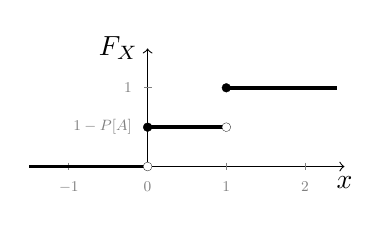
\begin{tikzpicture}
    \draw[->] (-1.5, 0) -- (2.5, 0) node[below] {$x$};
    \draw[->] (0, 0) -- (0, 1.5) node[left]{$F_X$};
    \foreach \x in {-1, ..., 2} {
        \draw [gray] (\x, 0.05) -- ++(0, -.1) ++(0, -.15) node [below, outer sep=0pt, inner sep=0pt, scale=0.6] {\small\(\x\)};}
    \foreach \y in {1} {
        \draw [gray] (0.05, \y) -- ++(-.1, 0) ++(-.15, 0) node [left, outer sep=0pt, inner sep=0pt, scale=0.6] {\small\(\y\)};}
    \draw [gray] (0.05, 0.5) -- ++(-.1, 0) ++(-.15, 0) node [left, outer sep=0pt, inner sep=0pt, scale=0.6] {\small\(1-\mathbb{P}[A]\)};
    \draw[draw=black,line width=1.3pt] (-1.5,0) -- (0,0);
    \draw[draw=black,line width=1.3pt] (0,0.5) -- (1,0.5);
    \draw[draw=black,line width=1.3pt] (1,1) -- (2.4,1);
    \filldraw[draw=black,line width=0.1pt,fill=white] (0,0) circle[radius=1.6pt];
    \filldraw[draw=black,line width=0.1pt,fill=black] (0,0.5) circle[radius=1.6pt];
    \filldraw[draw=black,line width=0.1pt,fill=white] (1,0.5) circle[radius=1.6pt];
    \filldraw[draw=black,line width=0.1pt,fill=black] (1,1) circle[radius=1.6pt];
\end{tikzpicture}

$F_X(x) = \begin{cases}
    0 & \text{if } x<0, \\
    1-\mathbb{P}(A) & \text{if } 0\leq x<1, \\
    1 & \text{if } x\geq 1.
\end{cases}$

2) Sei $X$ eine ZV mit cfd $F_X$. Sei $Y=exp(X)=e^X$. Dann ist $F_Y(x)=\mathbb{P}[Y\leq x]=\mathbb{P}[e^X\leq x]=\mathbb{P}[log(e^X)\leq log(x)]=\mathbb{P}[X\leq log(x)]=F_X(log(x))$. Weil $e^X>0$ $\forall x\in\mathbb{R} \Rightarrow \mathbb{P}[e^X\leq x]=0$ $\forall x\leq 0$. Somit erhalten wir
 
$F_Y(x) = \begin{cases}
    0 & \text{if } x\leq 0, \\
    F_X(log(x)) & \text{if } x>0.
\end{cases}$